% THIS IS SIGPROC-SP.TEX - VERSION 3.1
% WORKS WITH V3.2SP OF ACM_PROC_ARTICLE-SP.CLS
% APRIL 2009
%
% It is an example file showing how to use the 'acm_proc_article-sp.cls' V3.2SP
% LaTeX2e document class file for Conference Proceedings submissions.
% ----------------------------------------------------------------------------------------------------------------
% This .tex file (and associated .cls V3.2SP) *DOES NOT* produce:
%       1) The Permission Statement
%       2) The Conference (location) Info information
%       3) The Copyright Line with ACM data
%       4) Page numbering
% ---------------------------------------------------------------------------------------------------------------
% It is an example which *does* use the .bib file (from which the .bbl file
% is produced).
% REMEMBER HOWEVER: After having produced the .bbl file,
% and prior to final submission,
% you need to 'insert'  your .bbl file into your source .tex file so as to provide
% ONE 'self-contained' source file.
%
% Questions regarding SIGS should be sent to
% Adrienne Griscti ---> griscti@acm.org
%
% Questions/suggestions regarding the guidelines, .tex and .cls files, etc. to
% Gerald Murray ---> murray@hq.acm.org
%
% For tracking purposes - this is V3.1SP - APRIL 2009

\documentclass{sig-alternate}
\usepackage{amstext}
\usepackage{pdfpages}
\usepackage{alltt}
\usepackage{epstopdf}
\usepackage{xspace,colortbl}
\usepackage[USenglish]{babel}
\usepackage{multirow}
\usepackage{url}
\usepackage{subfigure}
\usepackage{graphicx}
\usepackage{amssymb}
\usepackage{fmtcount}
\usepackage{amsfonts}
\usepackage{xspace}
\usepackage{amsmath}
\usepackage{multirow}
\usepackage[mathscr]{eucal}
%\usepackage{psfrag}
\usepackage{colortbl}
\usepackage{bm}
\usepackage[nospace]{cite}
\makeatletter
\newif\if@restonecol
\makeatother
\let\algorithm\relax
\let\endalgorithm\relax
\usepackage[lined,boxed,vlined,ruled]{algorithm2e}
\usepackage[skip=1pt,font=bf]{caption}
\special{papersize=8.5in,11in}

\makeatletter
\def\@copyrightspace{\relax}
\makeatother

\begin{document}

\title{Social Influence Bias: A Non-Parametric Analysis of the California Report Card Rating Data}

\linespread{0.95}%
\setlength{\belowdisplayskip}{1pt} \setlength{\belowdisplayshortskip}{1pt}
\setlength{\abovedisplayskip}{1pt} \setlength{\abovedisplayshortskip}{1pt}
\selectfont

%
% You need the command \numberofauthors to handle the 'placement
% and alignment' of the authors beneath the title.
%
% For aesthetic reasons, we recommend 'three authors at a time'
% i.e. three 'name/affiliation blocks' be placed beneath the title.
%
% NOTE: You are NOT restricted in how many 'rows' of
% "name/affiliations" may appear. We just ask that you restrict
% the number of 'columns' to three.
%
% Because of the available 'opening page real-estate'
% we ask you to refrain from putting more than six authors
% (two rows with three columns) beneath the article title.
% More than six makes the first-page appear very cluttered indeed.
%
% Use the \alignauthor commands to handle the names
% and affiliations for an 'aesthetic maximum' of six authors.
% Add names, affiliations, addresses for
% the seventh etc. author(s) as the argument for the
% \additionalauthors command.
% These 'additional authors' will be output/set for you
% without further effort on your part as the last section in
% the body of your article BEFORE References or any Appendices.

\numberofauthors{3} %  in this sample file, there are a *total*
% of EIGHT authors. SIX appear on the 'first-page' (for formatting
% reasons) and the remaining two appear in the \additionalauthors section.
%\author{Sanjay Krishnan,Jay Patel,Ken Goldberg}

%

% Just remember to make sure that the TOTAL number of authors
% is the number that will appear on the first page PLUS the
% number that will appear in the \additionalauthors section.

\maketitle
\begin{abstract}
User-assigned ratings are a key component of almost all recommender systems.
Many rating systems show participants aggregate statistics from the community before they leave a rating.
These statistics can bias a participant's decision and is part of a broader class of biasing tendencies called Social Influence Bias.
We explore this bias in a new platform, the California Report Card (CRC), which reveals the median values to participants after they assign their own ratings, and then allows them to modify their ratings.
We hypothesized that this will lead to Social Herding, a type of Social Influence Bias, where participants change their ratings towards what they perceive as the norm.
We develop a non-parametric significance testing framework based on the Wilcoxon rank-sum statistic to test this hypothesis, and compare our results to a randomized SurveyMonkey survey asking the same questions as the CRC. 
We also propose a technique to test the effects of question order on social influence bias.
We learn a predictive model relating a participant's initial rating, the observed median, and the rating change, using a polynomial regression technique and Bayesian Information Criterion optimal model search.
Our results suggest statistically significant social herding towards the median value, and participants who changed their ratings were significantly more tightly concentrated around the median.
We learned the optimal polynomial model on ratings for six questions, four of which were modeled with linear functions indicating that homogeneity between a positive and negative social influence.
The two remaining questions, about the implementation of Obamacare and Same-sex Marriage Rights in California, were modeled as quadratic functions with significantly higher downward tendency for ratings higher than the median.
Our results suggest that using a predictive model to correct for the bias resulted in 46.5\% less herding around the median grade.
\end{abstract}

% A category with the (minimum) three required fields
%\category{H.4}{Information Systems Applications}{Miscellaneous}
%A category including the fourth, optional field follows...
%\category{D.2.8}{Software Engineering}{Metrics}[complexity measures, performance measures]

%\terms{Theory}

%\keywords{ACM proceedings, \LaTeX, text tagging} % NOT required for Proceedings

\section{Introduction}
Online tools increasingly rely on large amounts of data collected from the crowd.
For example, user-submitted product ratings in an e-commerce site can help recommend products to similar users in the future.
Rating data, like traditional surveys, are subject to a variety of biasing tendencies \cite{groves2013survey}.
We explore a class of biases, collectively called \emph{Social Influence Bias}, which arise from feedback from the actions of other users in the system \cite{demarzo2003persuasion, moscovici1972social, wood2000attitude}.
One aspect of Social Influence Bias is the phenomenon called \emph{social herding}, where the feedback from the community encourages future participants to conform to what they perceive as the ``norm" in the community.
The effects of social herding are crucial to the design of recommendation algorithms as many algorithms assume statistical independence between different users and use the spatial relationships between numerical features representing those users.

\begin{figure}[h]
  \centering
    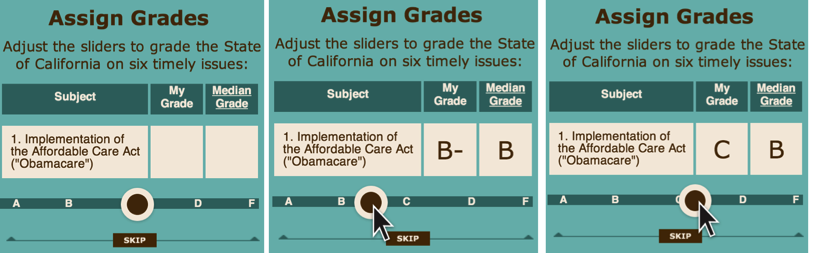
\includegraphics[width=\columnwidth]{../plots/grading-desc-1.png}
      \caption{Grading in the California Report Card. Participants enter grades on six timely issues facing the State of California. After entering their grades, the median grade over all participants is revealed. Participants have the option to change their grades after seeing the median. We model the tendency to regress towards the medians.}
      \label{grading-1}
\end{figure}

A common feedback mechanism is the use of aggregate statistics, for example, showing the average rating for a product before a participant shares his or her rating (Figure \ref{grading-1}).
In recent related work, Muchnik et al. \cite{muchnik2013social}, used a randomized experiment to determine the magnitude of social herding in up-voting in Reddit.com.
They randomly treated forum posts with extra up-votes and down-votes and measured the treatment effect; concluding that a statistically significant social herding tendency exists.
In this paper, we explore a related problem of whether users who have already submitted a rating will actually \emph{change} their existing ratings upon learning the median rating for the population and ``herd" towards the median grade.

As a case study, we use data from the California Report Card (CRC) \cite{crc}, where users graded the state of California on six timely issues.
After submitting a grade, users were shown the median grade of all other users.
We recorded any changes to previous grade that happened after the median was visible.
Such feedback of social content is an established technique to incentivize participation and increase user engagement with the tool \cite{shneiderman1992designing}.  
Furthermore, an application of particular interest is online participatory democracy where open aggregate results increase the transparency of the system \cite{albors2008new,o2012transparency,noveck2008wiki}.
For comparision with the CRC, we ran a reference survey through SurveyMonkey which was given to a random 611 participants from the company's paid pool of California participants.
In this survey, we asked users to respond to the same questions as the CRC on the same grading scale without the feedback of the median grade. 

The findings of Muchnik et al. suggest that social herding will be observed in the form of a regression towards the observed median grade during the grade changes.
In this paper, we test the hypothesis of social herding, propose a model for the relationship between observed medians and subsequent grade change, and provide experimental results comparing the data from the CRC to the randomized reference survey.

\subsection{Hypotheses and Contributions}
\noindent \textbf{Null Hypothesis} Viewing the median grade does not affect how a user chooses to change his or her grade, and does not affect any future grades given by the participant.

\noindent \textbf{Social Herding Around the Median} Grade changes are on average towards the median grade. Also, the final grades of participants who change their grades are more tightly concentrated around the median from participants who did not change their grades and participants from the reference survey.

\noindent \textbf{Social Herding and Question Order} Disagreement with the median on previous questions affect how a participant grades future questions. Participants who disagreed with the median greatly are more likely to leave future responses that are closer to the median. 

We develop non-parametric testing procedure, based on the Wilcoxon Rank-Sum statistic (also called the Mann-Whitney statistic) \cite{lehmann2006nonparametrics}, to test these hypotheses.
We chose a non-parametric framework because Muchnik et al. focused on only a binary input mechanism (up or down vote) and we extended this analysis to grading sliders with 13 possible vales from (A+ to F) without having to make strong assumptions about the distribution of grades.
In addition to the hypothesis testing, we model grade changes with a polynomial regression.
As before, to avoid having to make a strong assumption about the structure of the model, we use an information theoretic model to learn a flexibile degree polynomial.


\section{Related Work}

%% In the context of recommender systems, social influence has been studied primarily in order to use information about social and trusted friend networks to improve recommendations. Jamali et al. described a stochastic block model which predicts recommendations based on both social relations and rating behavior [A]. Shang et al. described models for for improving recommendations among individuals using the theory of social contagion, and among groups using network theory [B]. Ye et al. proposed a quantification metric of social influence, and proposed probabilstic model to model the decision of item selection [C].

%% However, the Asch model for confirmity suggest a particular biasing effect from an aggregate or ``crowd'' (i.e. the previous raters are anonymous to the current rater). This phenomenon known as social herding ...

The Asch model for conformity is the theoretical basis for what is sometimes called \emph{social herding}, the tendency to conform \cite{banerjee1992simple,bikhchandani2000herd}, and this has been a popular consumer choice model in economics \cite{burnkrant1975informational,dholakia2002auction,huang2006herding}. 
Such models have also been studied in psychology and behavioral economics as ``persuasion bias" \cite{demarzo2003persuasion, hong2004social, golub2010naive, dellavigna2009persuasion}.
In 2011, Lorenz et al. described how these biases can undermine the effectiveness of crowd intelligence in estimation tasks \cite{lorenz2011social}. 
They argue that movement towards the group consensus causes a diminished diversity of opinion potentially leading to inefficiencies and inaccurate collective estimates.
Danescu-Niculescu-Mizil et al. analyze helpfulness ratings on Amazon product reviews \cite{danescu2009opinions}.
They found that the helpfulness ratings did not just depend on the content of the review but also its aggregate score and its relationship to other scores.
In order to better distinguish social influence from other biases, Muchnik et. al designed a randomized experiment in which comments in an online forum were randomly up-treated or down-treated \cite{muchnik2013social}.
They concluded a statistically significant bias where a positive treatment increased the likelihood of positive ratings by 32\%. 
In both Danescu-Niculescu-Mizil et al. and Muchnik et al., they looked at the problem of social influence bias in an a priori setting, where users see the aggregate statistic before giving their rating.
Our work tests for a particular form of social influence where users are given the opportunity to change their opinions following the feedback. 

In recommender systems, Cosley et al. \cite{cosley2003seeing} studied the broad problem of biases in rating systems and tested the following relevant hypotheses:  can manipulated ``predicted" ratings influence a participant to change their rating, how consistent participants when re-rating an item, and how does rating scale (eg. stars, binary, unary) affect the average rating. 
The seminal result from Cosley et al. is that all of these hypotheses yeilded significant influencing tendencies.
We further study the propensity for bias in ``re-rating" to formulate an predictive model for a specific type of bias, social influence bias, and apply a nonparametric significance testing methology that is more robust to the discreteness and multimodality often observed in rating data.

Another line of relevant recommender systems research is the study of the consistency of repeat ratings \cite{amatriain2009rate, amatriain2009like}.
It is an open problem, how to incorporate models of noisy ratings into our framework, however, as our non-parametric significance test is rank-based it statisically robust to small amounts of random noise.
There has also been work on explaining recommendations \cite{bilgic2005explaining, tintarev2007survey}, and one way to evaluate these explanation systems is to give users the option to change their ratings and evaluate how much (or how little) the explanation changes the users rating.

Zhu et al. conducted an experiment in which users evaluate an image on a subjective question with binary scale (eg. ``Is this image cute?"), which was followed (either immediately or later) by a presentation of the crowd consensus opinion \cite{zhu2012switch}. 
Users were given an opportunity to change their response, and they concluded that there was a significant tendency to change submissions.
The tendency to change was the strongest when users were asked to make their second decision much later and not immediately after the first.
Along these lines, Sipos et al. argue that context along with an aggregate rating plays a large role in the users' ratings. That is, users may attempt to ``correct" the average, by voting in a more polarizing manner (more positively or negatively) \cite{siposreview}.
We extend this prior work to measure and predict these changes when the input is more complex than a binary scale, and propose a non-parametric methodology that can be, in principle, extended to a variety of different input mechanisms.
Our model can also account for a changing aggregate statistic such as a median rating changing as more data is collected. 


%% [A] M. Jamali, T. Huang, and M. Ester, ``A Generalized Stochastic Block Model for Recommendation in Social Rating Networks'', in ACM Conference in Recommender Systems (RecSys'11) , Chicago, IL, USA, October 2011.

%% [B] Shang, Shang, et al. ``Wisdom of the crowd: Incorporating social influence in recommendation models.'' Parallel and Distributed Systems (ICPADS), 2011 IEEE 17th International Conference on. IEEE, 2011.

%% [C] Ye, Mao, Xingjie Liu, and Wang-Chien Lee. ``Exploring social influence for recommendation: a generative model approach.'' Proceedings of the 35th international ACM SIGIR conference on Research and development in information retrieval. ACM, 2012.




\section{The California Report Card}
\subsection{System Description}
The California Report Card (CRC) is a web application that allows participants to advise the state government on timely policy issues.
When participants arrive at the application, they ``grade" the state on following six issues: (1) Implementation of the Affordable Care Act ("Obamacare"),
(2) Quality of K-12 public education, (3) Affordability of state colleges and universities, (4) Access to state services for undocumented immigrants, (5) Laws and regulations regarding recreational marijuana, and (6) Marriage rights for same-sex partners.
Grades are assigned on a thirteen point scale (A+,A,A-,...,D-,F).
These issues are posed in a fixed sequential order each with the same input scale.
Particpants submit grades using a click-and-drag slider interface as illustrated in Figure \ref{grading-1}.
On mobile devices this slider requires the participants to touch and drag their finger to the desired grade.

\begin{figure}[h]
  \centering
    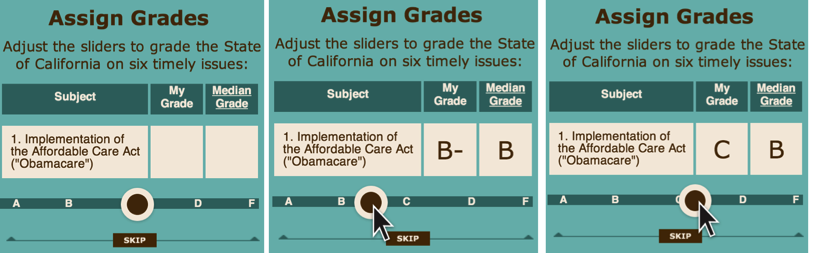
\includegraphics[width=\columnwidth]{../plots/grading-desc-1.png}
      \caption{Grading in the California Report Card. Participants enter grades on six timely issues facing the State of California. After entering their grades, the median grade over all participants is revealed. Participants have the option to change their grades after seeing the median.}
      \label{grading-1}
\end{figure}

Upon release of the slider, the CRC reveals the median grade for that issue over all prior participants.
Even after the median grade is revealed the slider is still active and participants can change their grades.
However, it is important to note that participants were not explicitly told that they could change their grades.
Another important observation is that participants who accessed the application at different times may have seen different median grades as they were calculated based on the data upto that point.
We recorded the initial grade, the median that the participant observed, and any subsequent changes along with timestamps for each of the events. 
Grading all of the six issues was not manditory and participant had the option to skip any of the issues.

The CRC has an additional open-ended discussion phase where participant submit textual suggestions on future issues to include in the report card.
In this work, we focus on the first phase and defer an analysis of biases in the discussion phase to future work.

\subsection{Notation}
To analyze this data, we mapped these 13 grades onto a scale from 0 to 1, with 1 being an A+ and 0 being an F.
Let $P$ denote the set of all participants.
For each participant $p_j\in P$, we associate a 3-tuple of grades ($g_i[j]$, $m[j]$, $g_f[j]$) which represent the initial grade, median observed by the participant, and the final grade.
For each issue, we divided the participants into three subsets of $P$: ones who did not change their grades $P_n$, ones who changed $P_c$, and ones who skipped the question $P_s$.
Our primary objective is to test the distributional properties of rating tuples from participants in $P_n$ compared to those in $P_c$.

To ensure that all participants in the set $P_c$ had an opportunity to see the median grade and then react, we filtered this group using the timestamps. 
The median grade appears in the interface with an animation whose completion time varied between devices, so we set a grace period of 3 seconds before 
we categorized the participant into set $P_c$.  

For consistency, we use the same notation to describe participants in the reference survey. We denote the set of reference survey participants as set $R$, and each participant is associated with a 3-tuple ($g_i[j]$, $m[j]$, $g_f[j]$). However, since the reference survey does not reveal the aggregate statistics $g_i[j] = g_f[j]$  and $m[j]$ is the median of the prior participants (which is not shown).

\section{Social Herding Towards the Median Hypothesis Test}\label{ht}
In this section, we test the \textbf{Social Herding Towards the Median} hypothesis, by analyzing spread of grades around the median grade for the participants that changed their grades.
There are three principle challenges in testing this hypothesis.
The first challenge is that parametric significance tests comparing two sample means such as the two sample t-test and z-test are known to 
perform poorly for multimodal and discrete distributions.
Another significance test that is commonly applied to compare spreads of distributions is the F-test, which is also known to perform poorly for many non-normal distributions \cite{markowski1990conditions}.
Furthermore, this test is usually used to test the spread of data around the mean, which only in very special conditions, such as normal distributions, aligns with the median which is relevant to our problem. 
The discretness of our data leads to mutli-modal distributions which are not optimal for these testing methods.

The second challenge is that there is a natural tendency for grades to concentrate around the median even without a bias.
Consider the following participant behavioral model.
Suppose that participants are not acustomed to a slider-based input.
We can model the first grade that the particpant leaves as uniformly randomly anywhere on the slider.
As the participant begins to understand how to use the slider their use becomes more accurate, ultimately settling on a grade from our observed distribution of final grades.
This model, the first grade is uniformly random and the second grade is a sample from the observed distribution, would result in a strong regression towards the median; even if there is no causal link with seeing the median.

Finally, the median grade $m_i$ can be different for each participant.
The median grade is calculated over all prior participants and thus is dependent on when the participant submitted their first grade.
In practice, the median will eventually converge for a large number of participants, but it would be incorrect to measure concentration around a final median.

To address these three challenges, we propose a non-parametric model based on the Wilcoxon statistic to test the hypothesis that the group of participants that changed their grades are more tightly centered around the median grade that the participants observed.
Our tests compare absolute deviations around the median for $P_n$, $P_c$, and $R$; which, as a relative test, controls for the natural tendency for grades group around the median.
Furthermore, it is more robust to the effects of alternate models such as the one described in our second challenge in comparision to a direct test of correlation.

\subsection{Non-parametric Significance Test}
Recall that $P_n$ is the set of participants that did not change their grades and $P_c$ be the set of participants that changed their grades.
We define a set $X_c,X_n$ of absolute deviations from the observed median of the final grade for each group:
\begin{equation}
X_c = \{|m[j] - g_f[j]|\}\text{ }\forall j \in P_c
\end{equation}
\begin{equation}
X_n = \{|m[j] - g_f[j]|\}\text{ }\forall j \in P_n
\end{equation}
For the purposes of hypothesis testing herding behavior, we ignore the sign of the deviation.
However, in Section \ref{changemod}, where we build a predictive model for the changes, we include the sign.

Now, for the set $X_c$, we calculate the Wilcoxon rank-sum statistic.
We assign a rank to each of the absolute deviations in the union set $\textbf{X} = X_c \cup X_n$ (ie. the largest change has rank 1 and the smallest has rank $|X_c \cup X_n|$.
For $X_c$, we sum the ranks of the deviations within its set:
\begin{equation}
W_c = \sum_{j \in P_c} R_j
\end{equation}

The \textbf{Null Hypothesis} is that absolute deviations in $X_c$ are the same size as $X_n$. 
Under this null hypothesis $median(X_n) = median(X_c)$, the ranks will be evenly distributed between each group. 
Therefore, the null expected value and variance of $W$ is:
\begin{equation}
\mathbb{E}(W) = \frac{(|\textbf{X}| + 1)\cdot |X_c|}{2}
\end{equation}
\begin{equation}
var(W) = \frac{(|\textbf{X}| + 1)\cdot |X_c| \cdot |X_n|}{12}
\end{equation}
For the significance level $\alpha$, we can test the probability that our calcuated $W_c$ comes from the null distribution.
In other words, the test calculates the probability that a random subset of users (ignoring the categorization $P_n$ and $P_c$) can have the observed difference in rank-sum values.
A significant result means that for the participants that changed their grades the changed changes are more tightly centered around the median grade they observed.

The same analysis can be used to test $X_c$ against the absolute deviations in the reference survey $X_r$
\begin{equation}
X_r = \{|m[j] - g_i[j]|\}\text{ }\forall j \in R
\end{equation} 
or for initial vs. final ratings in the change group $X_c'$:
\begin{equation}
X_c' = \{|m[j] - g_i[j]|\}\text{ }\forall j \in P_c
\end{equation}

\subsection{Quantifying Concentration of Grades}
In addition to testing the hypothesis, we can also quantify the effects of social herding. 
We tested the significance of the absolute deviations using a Wilcoxon test statistic.
The Wilcoxon statistic can be inverted to estimate a most likely \emph{shift parameter}, that a constant shift $\Delta$ in the distribution of absolute deviations $X_c$ that maximally aligns them with $X_n$ (ie. $X_c + \Delta$ is most supported by the null hypothesis). 
Since $X_c$ is a set of absoulte deviations, $\Delta$ tells us how much more concentrated $X_c$ is than $X_n$ around the observed medians.
This parameter is relevant to the design of recommendation algorithms use proximity (eg. clustering or nearest neighbors).

We refer to \cite{lehmann2006nonparametrics} on the derivation of $\Delta$ and its confidence interval:
\begin{equation}
D = \{x_n[j] - x_c[i]\} \text{ } \forall i,j \in X_n, X_c
\end{equation}
\begin{equation}
\Delta = median(D)
\end{equation}

%\subsection{Discussion About the Grade Distribution}
%In Figure \ref{dist-1}, we show the distribution of absolute deviations for the Marriage Rights issue. 
%\begin{figure}[ht!]
%  \centering
%    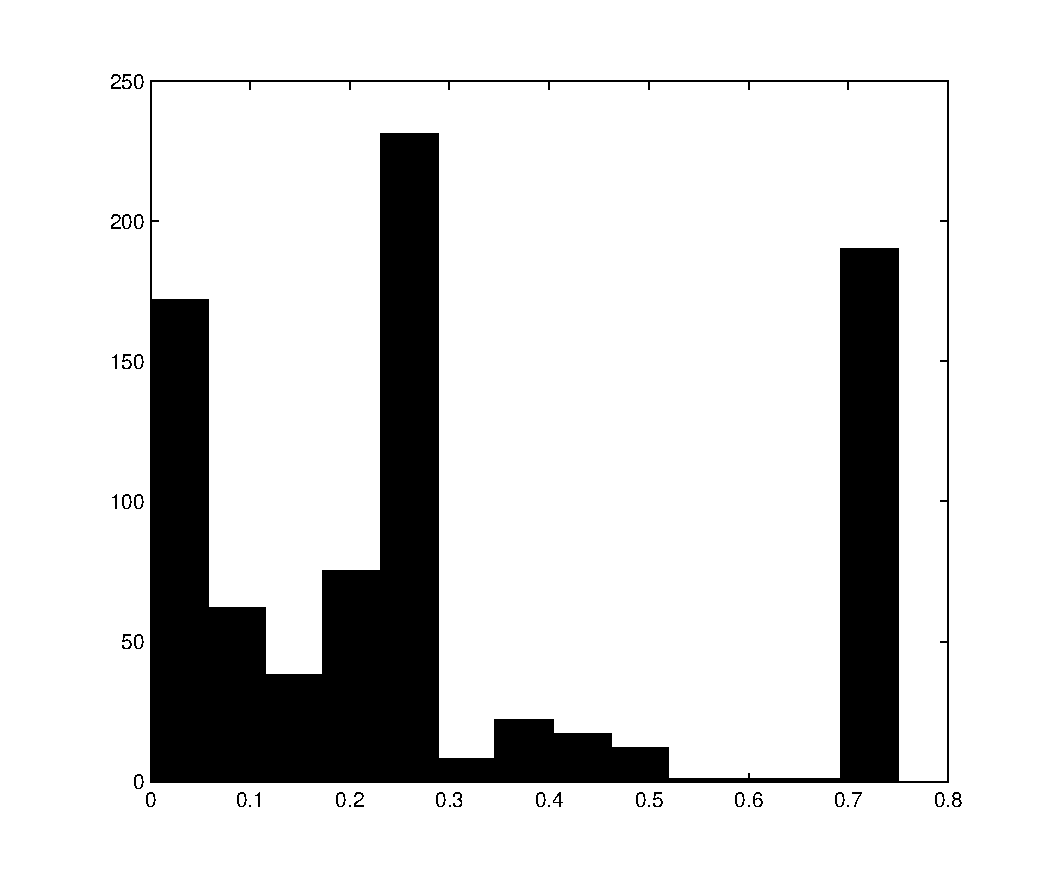
\includegraphics[scale=0.40]{../plots/absolute-deviations.eps}
%      \caption{\textbf{TODO}}
%      \label{dist-1}
%\end{figure}
%We see that the distribution is multimodal and discrete. 
%Parametric tests such as the z-test and the t-test have been shown to have weaker statistical power in many families of multimodal distributions such as mixtures of Gaussians \cite{???}.
%Rank-based tests tend to be more robust to the multimodality and in fact don't depend on the actual values on the relative frequency of the ranks in the test set.




\section{Social Herding and Question Order}
\label{path}
In this section, we develop a model for testing the effect of the sequence of ratings.
Order effects have been well studied in surveying \cite{krosnick1987evaluation}, and we look at order effects in the context of social herding. 
Recall, that we posed the each of the six questions in a fixed order.
Our question of interest is: given a participant's average disagreement with the median grade (measured by the absolute deviation) on the previous issues, how is their grade to the following issue affected?
We hypothesize that participants will become more moderate in their grades if they observe that their grades a consistently in disagreement with the population consensus.

This hypothesis is challenging to test as responses to issues may be correlated; even excluding any form of bias.
Consider the following example, if the grades are positively correlated, then low grades on one question could imply even lower grades on another.
In this case, we would see an increase in deviations even though it is not attributable to the biasing tendency.
Consequently, we build a model that compares the CRC to the SurveyMonkey reference survey.
We test to see if the relationship between the deviation of a participant's past grades and their current grades is different between the CRC and reference survey.

Let $d_{kj}$ be the absolute deviation from the median grade of participant $j$'s grade on issue $k$. 
We define a statistic $\bar{d}_{kj}$, which is the mean of all of the absolute deviations on the previous issues:
\begin{equation}
\bar{d}_{kj} = \frac{1}{k-1} \sum_{l < k}  d_{lj}
\end{equation}
If an issue was skipped by participant $j$, we exclude it from the average.
For each issue $k > 1$, we can get a set of differences between the absolute deviation of the current issue and $\bar{d}_{kj}$:
\begin{equation}
D_k = \{(\bar{d}_{kj}-d_{kj})\} \forall j
\end{equation}
We can calculate the same set of deviations for the reference survey which we call $D_k^{(r)}$.
When the differences in $D_k$ are on average positive it means that on issue $k$ participants were more moderate than previous issues and vice versa if the differences are negative.
So formally, our hypothesis test compares whether the set of differences in the CRC $D_k$ are larger than the set of differences in the reference survey $D_k^{(r)}$.
A significant result means that in comparison to the reference survey, CRC participants showed a greater tendency to center their grades around the median after disagreeing on previous issues.

We can apply the same Wilcoxon rank-sum model discussed in the previous section to test this hypothesis.
The testing procedure is the following: (1) we rank the differences in $D_k \cup D_k^{(r)}$, (2) we calculate $W$ which is the sum of the ranks in $D_k$, and 
(3) using the equation from the previous section we test the calculated W under the null hypothesis distribution.
The null distribution models the null hypothesis that there is no difference between $D_k$ and $D_k^{(r)}$, and given this hypothesis what is the probability we will observe the rank-sum statistic $W$.

This test is particularly interesting in the context of initial grades.
If we construct our set $D_k$ so that $\bar{d}_{kj}$ is based on final grades and $d_{kj}$ is the deviation of the initial grade, we can test to see how the concentration of grades around the median changes even without the biasing effect of revealing the median.
The implications of this question are interesting since this tests whether participants have a tendency to \emph{guess} the median grade after prior disagreement with the median.

\section{Predicting Magnitude of Grade Changes}
\label{changemod}
In the previous two sections, we proposed a technique to test the significance of the social herding hypothesis.
In this section, we build a model to describe the relationship between the variables in the 3-tuple ($g_i[j]$, $m[j]$, $g_f[j]$).
In other words, given a participant's current grade, the median they observed, can we predict the final grade?

\subsection{Modeling Changes}
Previous work, suggests that Social Influence is not a homogenous bias, namely, positive influences are different from negative influences.
In Muchnik et al. \cite{muchnik2013social}, they found that when they positively treated posts with higher up-vote counts in Reddit it lead to a significant increase in the likelihood of additional up votes (32\% more likely). 
On the other hand, they argue negative treatments inspired correction behavior; where some participants wanted to correct what they felt was an incorrect score. 
They found that this also increased the likelihood of up-voting (88\% more likely); as opposed to the herding response which would be increased down-votes.

These results suggest that the effects of viewing median grades can be non-linear and are very context/question dependent.
Similar to the previous section where we applied non-parametric tests that did not make a strong assumption about the distribution of the data, we propose a information theoretic model search that allows flexible parameter selection without making strong assumptions about the nature of the relationship.
Conditioned on the event that the participant changes their grade, we learn a functional relationship between the observed median and initial grade that can be a polynomial of any degree.
While the space of all polynomial models is fairly exhaustive, we acknowledge that this model can only fit curves that are continous and smooth.

Let $f\in \mathcal{P}^k$ be a polynomial of degree $k$.
The square loss of $f$, is the error in predicting $g_f[j] - g_i[j]$ from $f(m[j] - g_i[j])$:
\begin{equation}
\mathcal{L}(X_c;f,k) = \sum_j ((g_f[j] - g_i[j]) - f(m[j] - g_i[j]))^2 
\end{equation}
For a given $k$, the best-fit polynomial minimizes this square-loss:
\begin{equation}
f^*_k =\arg \min_f \mathcal{L}(X_c;f,k)
\end{equation}
For a given $k$, this problem can be solved with least squares.
To search over the space of polynomial models, we apply a well-studied technique called the Bayesian Information Criterion (BIC) \cite{schwarz1978estimating,burnham2002model}.
This technique converts the optimization problem into a penalized problem that jointly optimizes over the ``complexity parameter" k.
This penalty can be interpreted as bias towards lower degree models, in other words, an Occam's Razor prior belief. 
Cross-validation is an alternate method to empirically determine optimal model, and in practice, they give very similar results.
BIC, however, is derived through maximum likelihood estimate and is not an empirical so the learned model has a notion of optimality conditioned on the BIC prior belief.

Thus, we reformulate the optimization problem in the following way to incorporate the BIC penalty:
\begin{equation}
\arg \min_{f,k} |X_c|\log(\mathcal{L}(X_c;f,k)) + k\log(|X_c|)
\end{equation}
The resulting optimal polynomal will tell how the regression affects varies as a function of $m[j] - g_i[j]$ while controlling for over-fitting to our data.
In general, this optimization problem is non-convex so we incrementally try polynomials of degree 1,2,3.. etc. until we reach a local minimum.

\section{Results}
We evaluated our models on data collected from the California Report Card between January 18th to April 20th.
We adminstered our reference survey through SurveyMonkey between March 8th and March 14th.
We consider a set of 1575 total participants from the CRC and a sample of 611 SurveyMonkey participants whose grading activity was as follows:\\[1\baselineskip]

{\centering\scriptsize
\begin{tabular}[!ht]{ l | r | r | r | l }
Issue & No Change & Change & Skip & Median \\
\hline
\hline
  \multicolumn{5}{l}{\textbf{CRC}}\\
  \hline
  Obamacare & 749 & 223 & 593 & B \\
  \hline
  K12 & 849 & 172 & 544 & C+ \\
  \hline
  College & 923 & 139 & 503 & C-\\
  \hline
  Immigration & 693 & 105 & 767 & C \\
  \hline
  Marijuana & 881 & 118 & 566 & C \\
  \hline
  Marriage Rights & 929 & 105 & 531 & B+\\
\hline
\hline
\multicolumn{5}{l}{\textbf{Reference}}\\
\hline
  Obamacare & 498 & - & 113 & B \\
  \hline
  K12 & 561 & - & 50 & C \\
  \hline
  College & 573 & - & 38 & C-\\
  \hline
  Immigration & 375 & - & 236 & C+ \\
  \hline
  Marijuana & 498 & - & 113 & C \\
  \hline
  Marriage Rights & 554 & - & 57 & B+
\end{tabular}\\[1\baselineskip]
}

For any given issue, between 10\% and 20\% of those who assigned grades registered a grade change.
In all, 556 out of the 1575 CRC participants changed their grades at least once (Figure \ref{change-1}).
We also found that the aggregate results of the reference survey matched the CRC quite well.
On only two issues (K12 and Immigration), we found a observed differences which were both less than a letter grade (+ or -).
\begin{figure}[h]
\vspace{-1.5em}
  \centering
    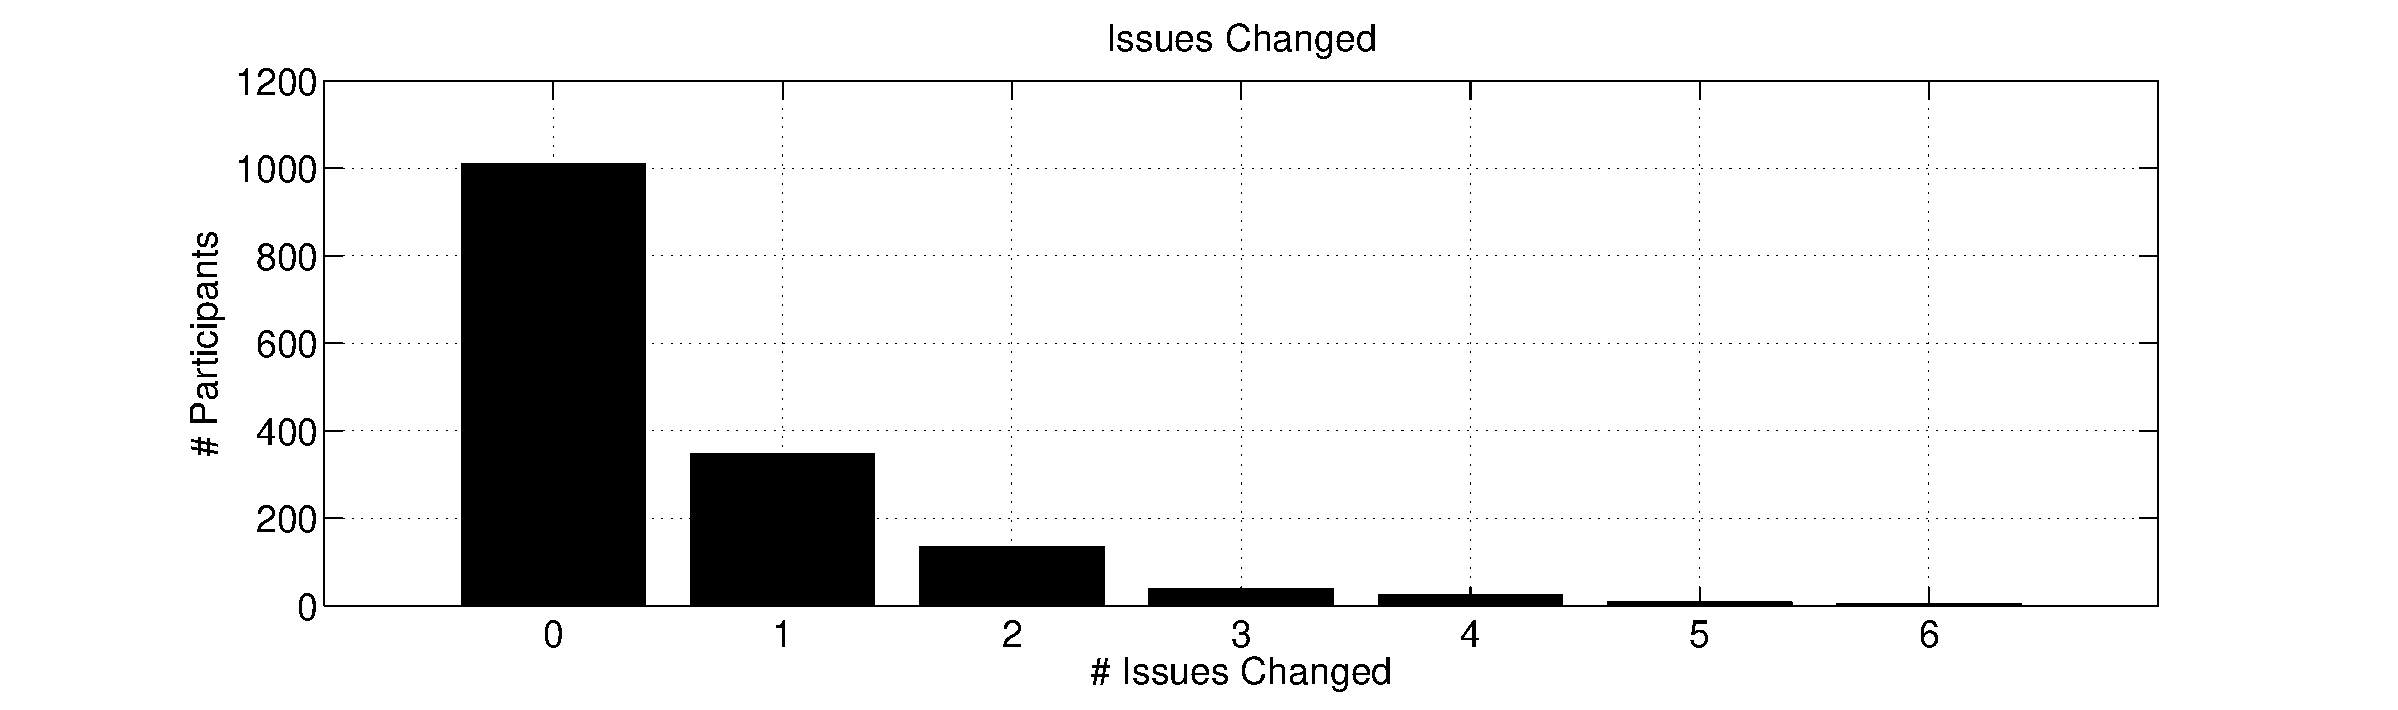
\includegraphics[scale=.28]{../plots/change-1.eps}
      \caption{The majority of participants did not change grades. 35\% of participants changed their grade on at least one issue, the majority of which (62\%) changed only a single issue. Less than 5\% of participants changed their grades on more than 4 out of the 6 issues.}
      \label{change-1}
\end{figure}
In our evaluation of these two surveys, we will use the unit \emph{full letter grades}.
For example, one full letter grade corresponds to the difference between an A grade and a B grade. 
A difference of a + or - is represented as $\frac{1}{3}$ eg. B to B+ or B+ to A-. 
\subsection{Social Herding Towards the Median}
Using the non-parametric test proposed in Section \ref{ht}, we tested the hypothesis of whether grade changes led to significantly more concentration around the median grade.
In our first experiment (Figure \ref{mdev-1}), we tested the absolute deviations of only the CRC participants.
We compared the group of participants that did not change their grades to the group that changed their grades.
We found that while there were no statistically significant differences between the initial grades of the two groups, the final grades of the group that changed were statistically significantly more concentrated than both their own initial grades and the grades of the no change group.
For the set of participants who changed their grades $P_c$ and those who did not $P_n$:
\begin{figure}[h]
\hspace{-2em}
    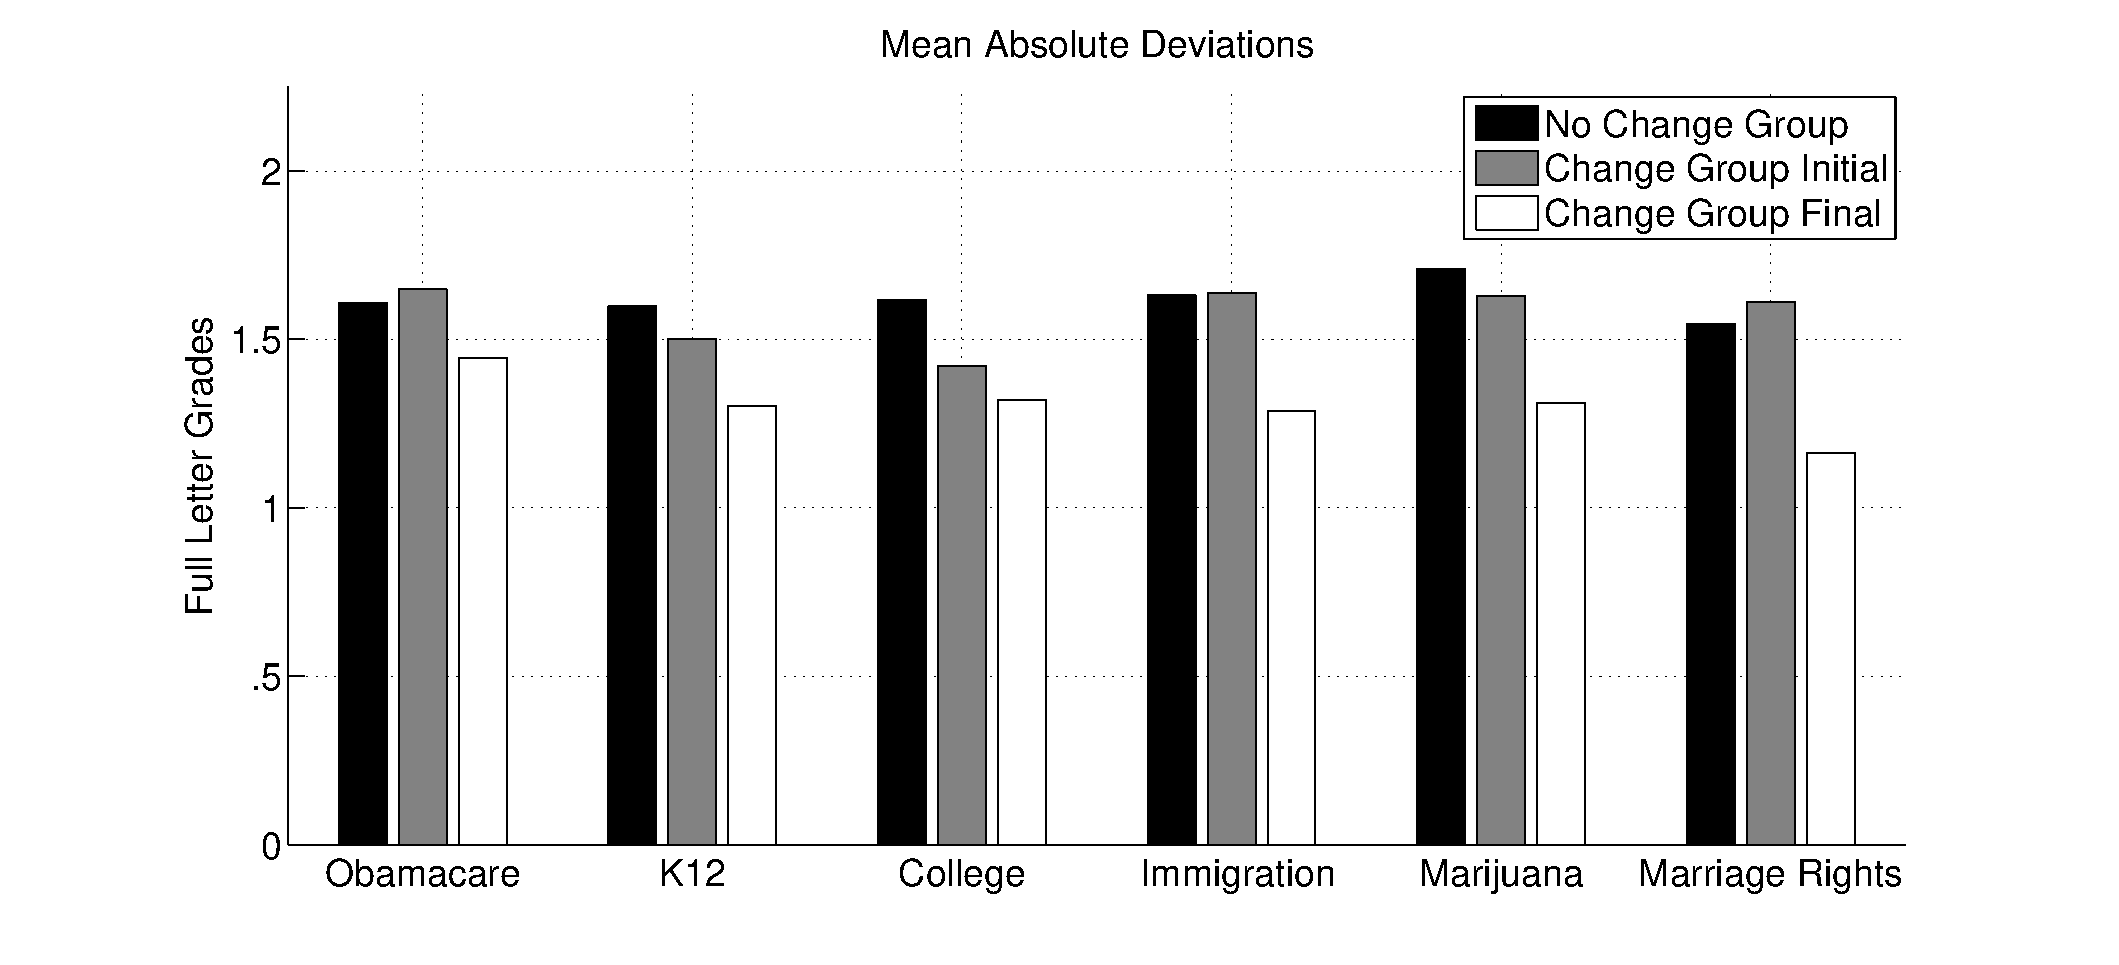
\includegraphics[scale=0.27]{../plots/abs-deviations-1.eps}
      \caption{For those participants that changed their grades, final grades were significantly more concentrated around the median grade than their initial grades. In addition, these grades are more concentrated than the grades for those who didn't change.}
      \label{mdev-1}
\end{figure}

{\centering
\scriptsize
\begin{tabular}[!ht] { r | r | r }
\label{dev-2}
  Issue & p-val($P_c$ vs. $P_n$) & p-val($i$ vs. $f$) \\
  \hline
  \hline
  Obamacare &  0.0286 & 0.0161 \\
  \hline
  K12 & 2.1314e-06 &  0.0086 \\
  \hline
  College & 1.3033e-04 & 0.0415 \\
  \hline
  Immigration & 7.3456e-07 &4.4170e-05\\
  \hline
  Marijuana & 2.7549e-10 & 4.2560e-05\\
  \hline
  Marriage Rights & 3.5946e-06 & 2.4644e-10 \\
\end{tabular}\\[1\baselineskip]
}

These results are consistent with the social herding hypothesis.
When participants change their grades, they are more likely to concentrate around the median.
What is particularly surprising is that the two groups of participants $P_n$ and $P_c$ are very similar in terms of intial grades, and the data suggests that herding is not correlated with more or less concentrated initial grades.

In our second experiment (Figure \ref{mdev-2}), we apply the same testing procedure to compare the grades from the CRC to to those in the reference survey.
We absolute deviations of the group of participants who changed their grades in the CRC against participants from the reference survey.
\begin{figure}[h]
\hspace{-2.6em}
    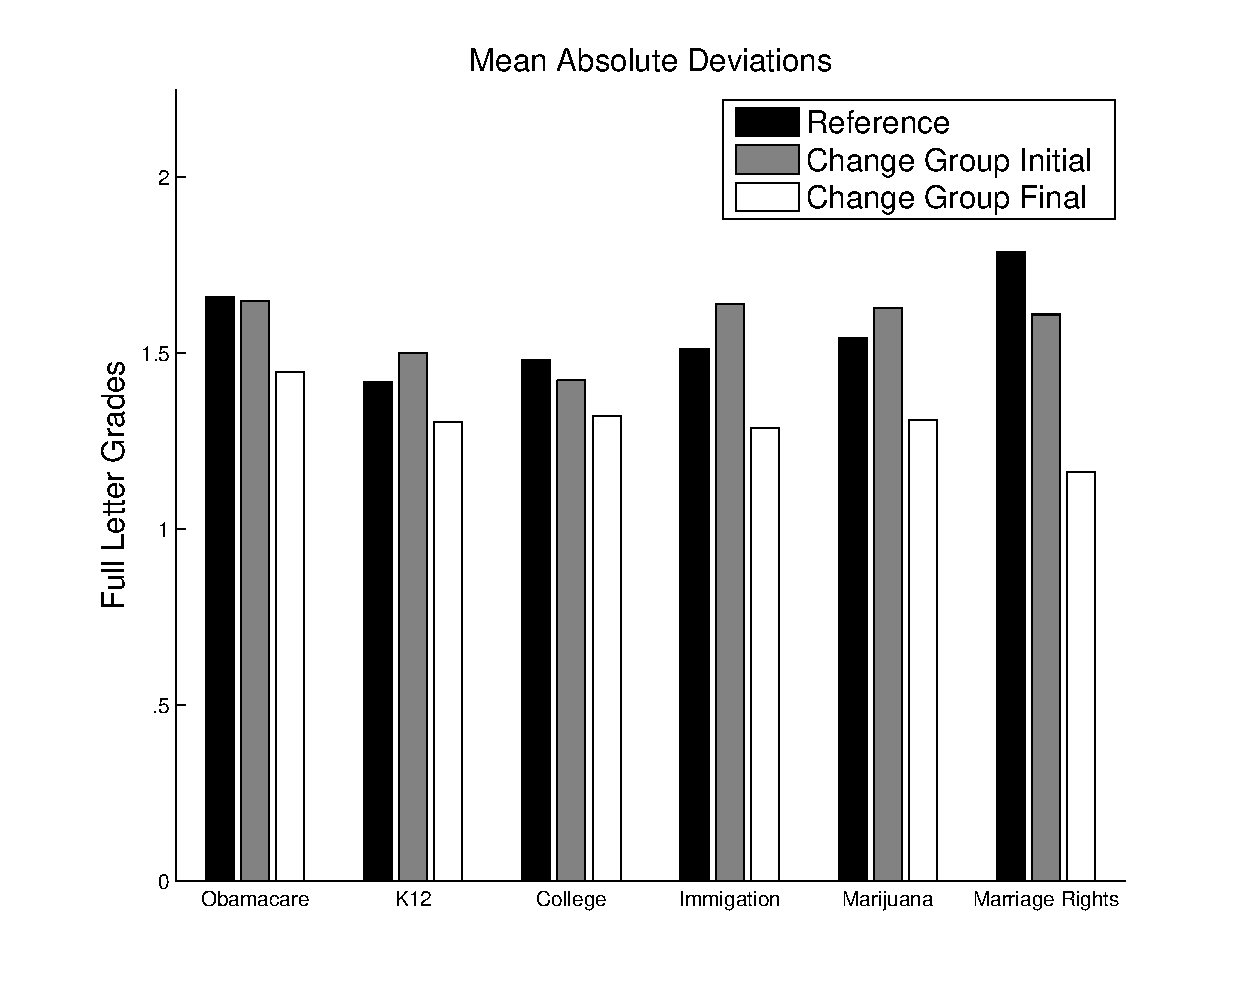
\includegraphics[scale=0.27]{../plots/bias-2.eps}
      \caption{We found that final grades were significantly more concentrated in the CRC compared to grades in the reference survey. Similar to Figure \ref{mdev-1}, we found that there was no statistically significant difference between the reference survey and the initial grades.}
      \label{mdev-2}
\end{figure}

{\centering
\scriptsize
\begin{tabular}[!ht] { r | r | r }
\label{ref-1}
  Issue & p-val($R$ vs. $i$) & p-val($R$ vs. $f$) \\
  \hline
  \hline
  Obamacare &  0.5386 & 0.0015 \\
  \hline
  K12 & 0.8283 & 0.0097 \\
  \hline
  College & 0.1452 & 0.0091 \\
  \hline
  Immigration & 0.3765 & 1.1787e-04\\
  \hline
  Marijuana & 0.7288 & 9.3111e-06\\
  \hline
  Marriage Rights & 0.2478 & 0.0161 \\
\end{tabular}\\[1\baselineskip]
}

The results of our two experiments suggest that the CRC rating data is affected by social herding.
We not only found that participants' changed grades were statistically significantly more likely to concentrate around the median, they were also more likely in comparision to the reference survey.
While correlation does not imply causation, we argue that this evidence is most consistent with the social herding hypothesis.
As the CRC was not a randomized survey, there are possibly confounding covariates eg. participants who changed their grades were more likely to leave tightly concentrated grades in the first place.
However, our comparision with the reference survey, and discovery that initial grades were largely consistent with the reference survey and with those that didn't change their grades, suggest that these confounding covariates are not very significant.
These results are encouraging and we hope to run a randomized participant study to confirm the causal relationship between revealing the median and concentrated grades.

\begin{figure}[ht!]
\centering
  \hspace{-3em}
    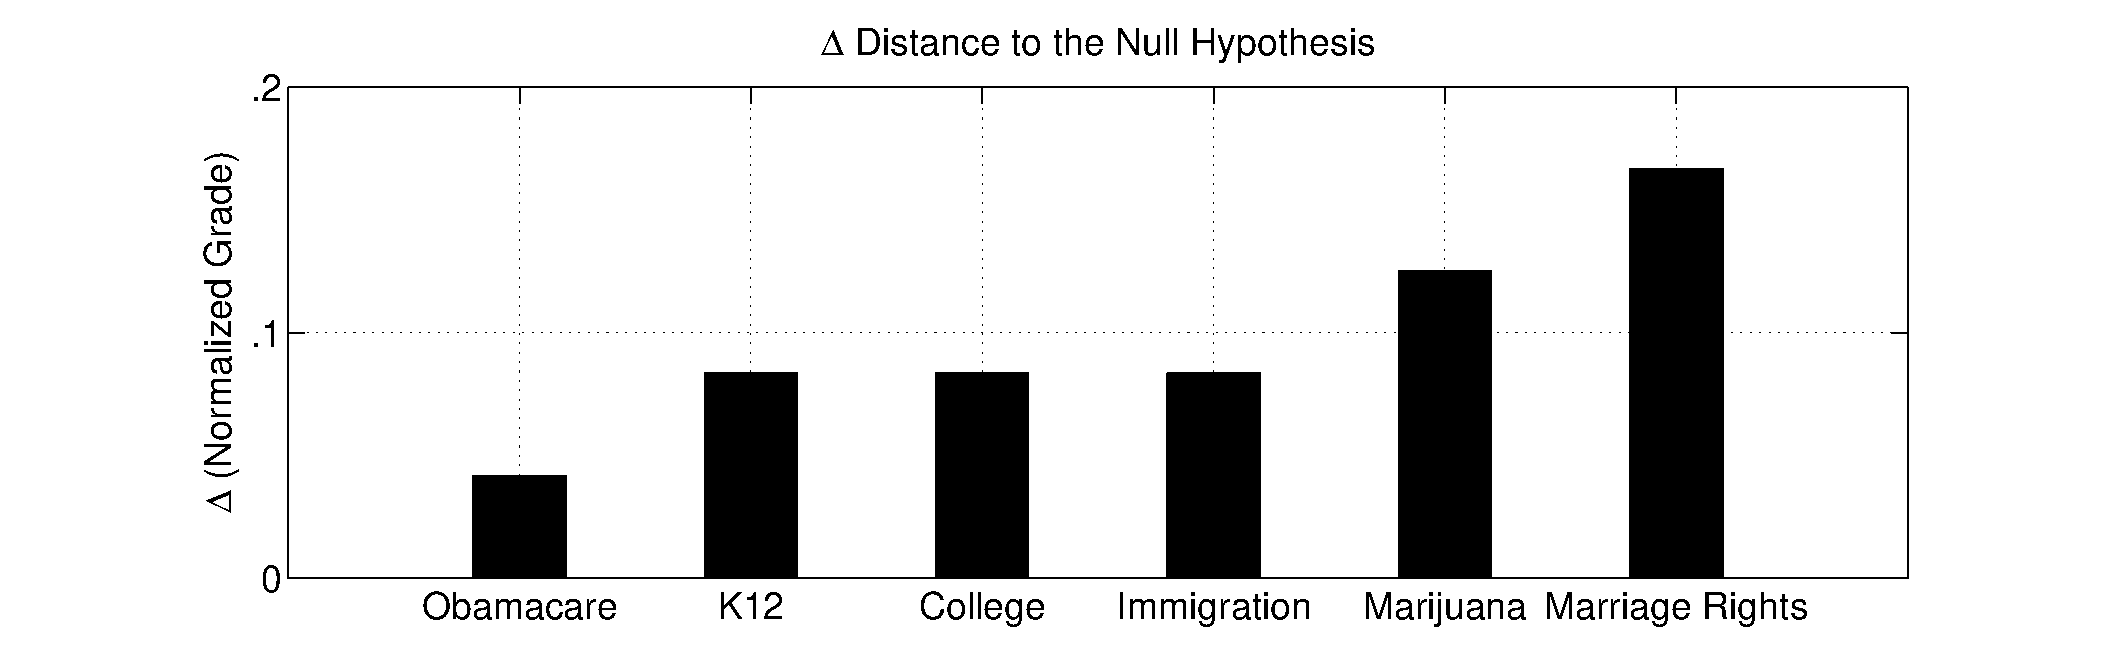
\includegraphics[scale=0.25]{../plots/shift-parameter.eps}
      \caption{We calculate the parameter $\Delta$ which is the most likely amount that our observations deviate from the null hypothesis. This can be interpreted as how much more are grades in our change group concentrated around the median.}
      \label{shift-1}
\end{figure}
\subsection{Social Herding Effects}
We tested the hypotheses and conclude significant additional concentration of grades around the median grade.
In Section \ref{ht}, we described how we could use the results of the hypothesis test to estimate the $\Delta$ parameter, which quantifies how different the hypothesis is from the null distribution.
In Figure \ref{shift-1}, we show the parameter estimates for each of the issues.
As before, the units of the plot are in terms of letter grades.
For the issues about Marriage Rights, we find that parameter is 2/3 of a letter grade.
This means that the set of absolute deviations for the change group $X_c$ was on average 2/3 of a letter grade smaller.
For the other issues, the parameter was smaller indicating less of an effect of social herding.
The parameter was the smallest for the first issue (Obamacare), and we conjecture that for this issue many participants were still learning how to use the slider interface; leading to random grade changes.
For this issue, we see that it had the most number of grade changes as well.

This parameter is very relevant to the design both recommender systems and predictive models.
Consider the problem of trying to predict a particpant's next grade.
The simplest model we could design is a model where we always select the median grade.
Such a model is often used as a baseline for comparision in recommender systems.
What we may interpret as low prediction error may in fact be the effects of social herding around the median, and if we were to apply this model asking the same questions but in a system without the herding effects; we may find that the same model performs poorly.
A median prediction is a naive model, but this problem affects many recommendation algorithms since they often rely on proximity metrics such as clustering, k-nearest neighbors, and some kernel machine learning methods.
\subsection{Order Dependence and Social Herding}
Using the model proposed in Section \ref{path}, we calculated the test statistics for both the CRC and the Reference Survey.
Recall, that this model calculate the change in disagreement with the median; that is, how much did a participant disagree with the median on past responses compared 
to the current value.
A comparatively larger value in the CRC suggests repeated feedback of the median grade encourages future responses to be more moderate.
Figure \ref{path-1} illustrates the results of the experiment for the five last issues (K12, College, Immigration, Marijuana, Marriage Rights), and using the mean disagreement on the previous issues.
The experimental results were not as significant as the other experiments and we found that only two issues Immigration (p=0.0037) and Marijuana (p=0.0287) showed an order dependence that was significantly greater than the reference survey.
For the other issues it is not clear if and how order plays a role in the social herding bias.
\begin{figure}[h]
	\hspace{-2em}
    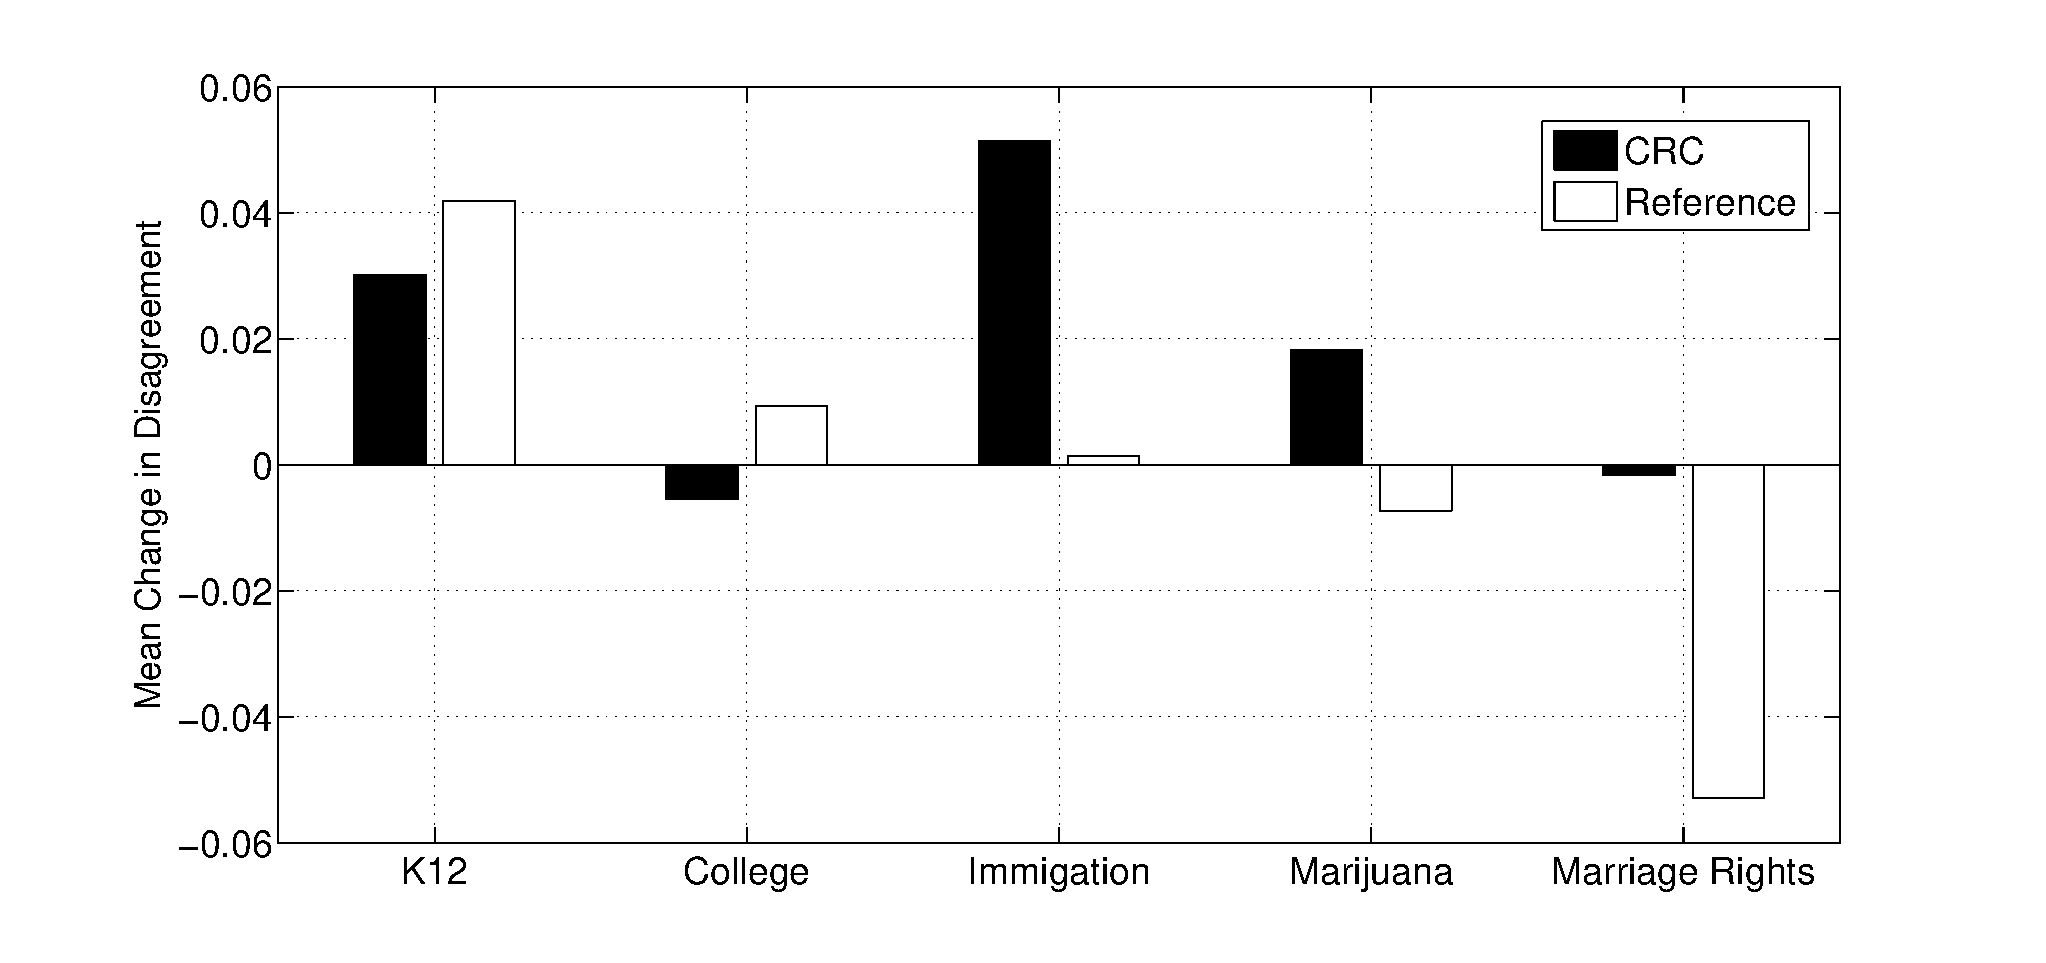
\includegraphics[scale=0.27]{../plots/path-dependence.eps}
      \caption{We measure the mean change in disagreement for each issue. The change in disagreement is defined as the average deviation with median on previous issues minus the deviation with the median on the current issue. We hypothesized that the CRC would have comparatively greater (or less negative) values than the reference survey.}
      \label{path-1}
\end{figure}
In summary, we were not able to reject the null hypothesis for order dependence, but we did find some indication with two statistically significant results that it plays an important role.
This underscores the subtlty social herding and social influence bias as they are very question and context dependent.

\begin{figure*}[ht!]
\hspace{-7em}
    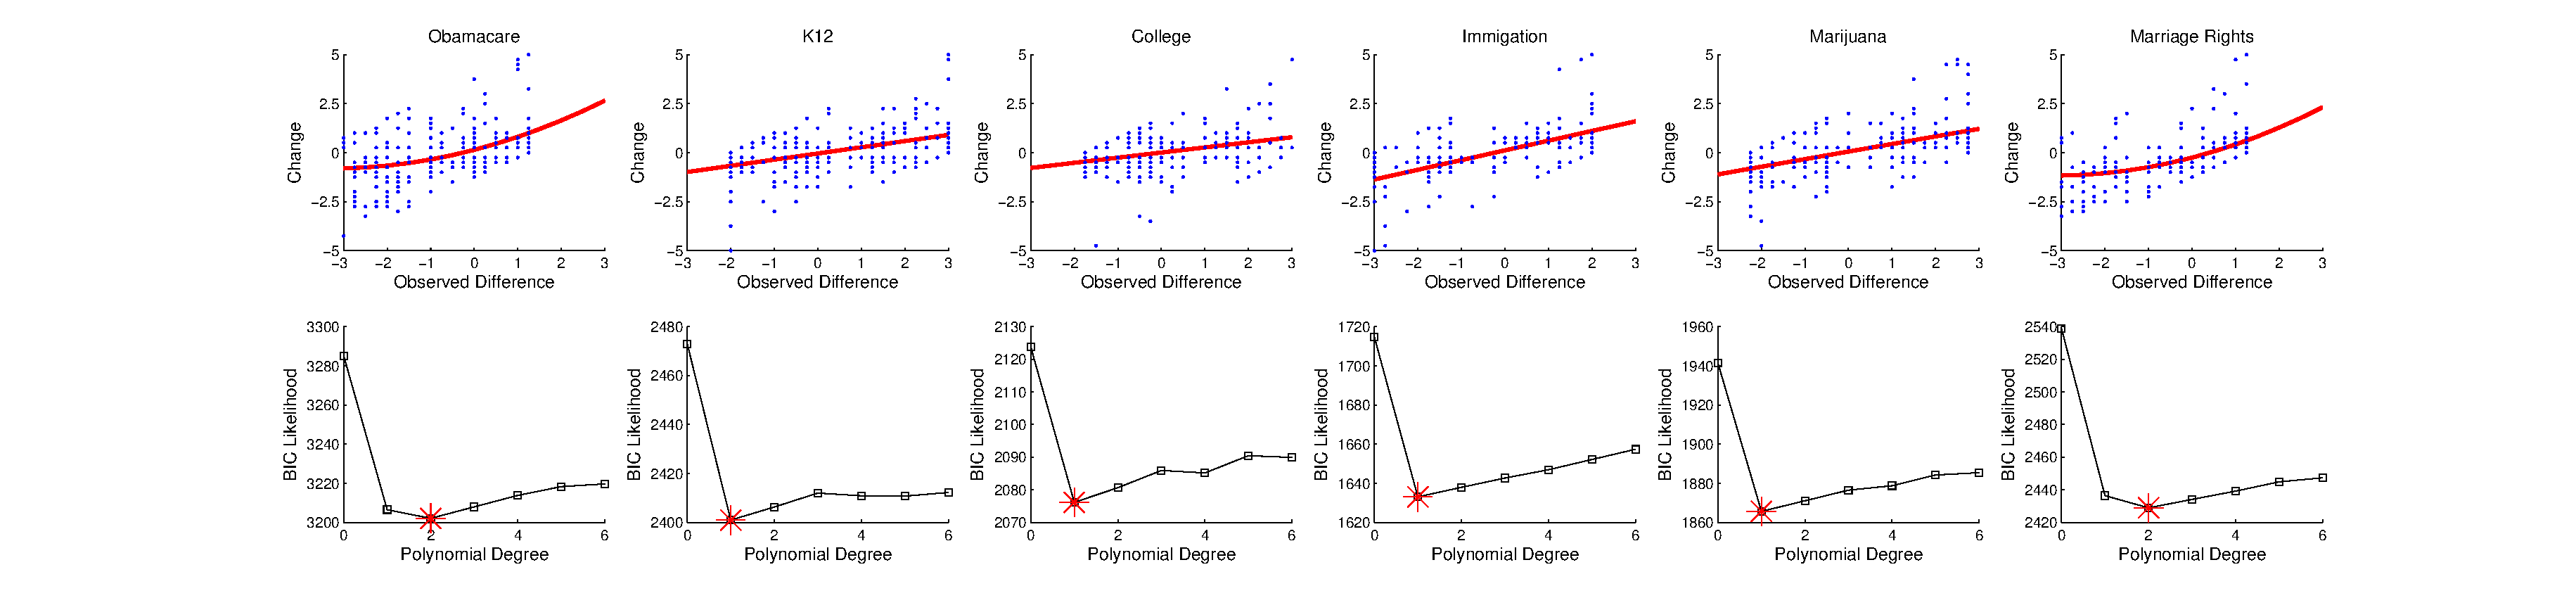
\includegraphics[scale=0.36]{../plots/BIC-optimization.eps}
      \caption{For the participants that changed their grades, we plot the difference between their grade and the median (X-axis), and their changed grade (Y-axis). We overlay the optimal polynomial model to represent the relationship $f(x) = y$. Below each plot, is the BIC objective function showing how we picked an optimal degree of polynomial.}
      \label{opt-1}
\end{figure*}
\subsection{Predicting Grade Changes}
We train the polynomial model proposed in Section \ref{changemod}, and the results are shown in Figure \ref{opt-1}.
Our model search and optimization through the BIC discovered that for four out of the six issues, K12, College, Immigration, and Marijuana, the model was linear.
This suggests homogeneity in positive and negative social influence effects for these issues.
However, for Obamacare and Marriage Rights, we found that the relationship was quadratic.
Interestingly enough, over the domain of changes, the learned quadratic was ``almost" linear, however it modeled heterogeneity in positive and negative influence effects.
Participants who initially graded the state higher than the median had a more significant tendency to change downwards, in comparision to the upward tendency of those who graded less than the median.

These models further illustrate the subtlty of social influence bias. 
In Muchnik et al. they observed a biasing tendency where both positive and negative influence led to increased upward bias (due to herding and correcting tendencies respectively).
Compared to those results, our results are quite different as we observe herding for both positive and negative influences.
One possible explanation is that since our mechanism for social influence is revealing the true grade, not modifying the grade (thus showing an ``incorrect" value), the correcting tendency is not significant.

We also tested our model in terms of RMSE prediction error (Figure \ref{poly-1}). 
We held out 20\% of the pairs of ratings (observed change, actual) and tested the prediction error on this held out set.
We found that our model on average, over all issues, predicted final grade within $0.5150$ letter grades.
Note that 1/3 of a letter grade corresponds to the difference of just a + or - grade.

We can further look at the \emph{inverse} model performance, that is, inverting the polynomal regression where we predict the change amount given the final grade and the median.
In a second experiment (Figure \ref{poly-1}), we re-calculated the shift-parameter $\Delta$ after applying the inverse model correcting for the social herding.
We found that there was on average a 46.5\% reduction in $\Delta$ which quantifies the herding around the median. 
This suggests that our predictive model can significantly mitigate the effects of social herding.

Consider the following application of such a model.
If we have collected rating data that we suspect is affected by Social Influence Bias towards a revealed aggregate statistic.
We can run a controlled experiment offline to collect training data that collects initial and final ratings.
We can fit our polynomial model to that data and apply the model to correct our bigger dataset.
The corrected data will more accurately reflect the spread of ratings around the aggregate statistic mitigating the herding around the revealed value.

\begin{figure}[h]
\hspace*{-2em}
    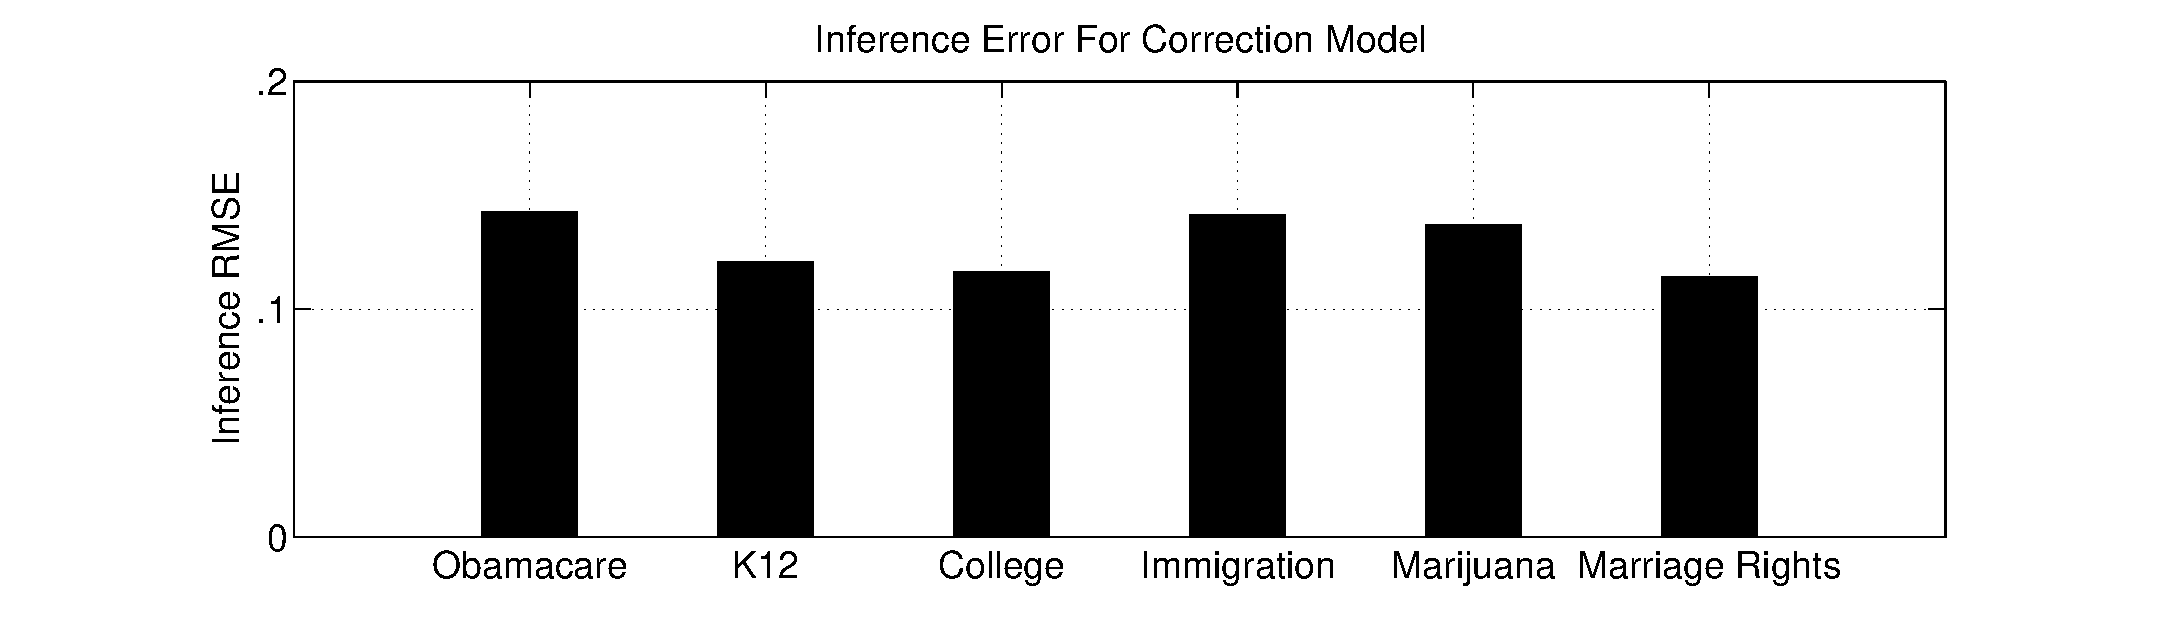
\includegraphics[scale=0.26]{../plots/prediction-error.eps}
    \hspace*{-2em}
    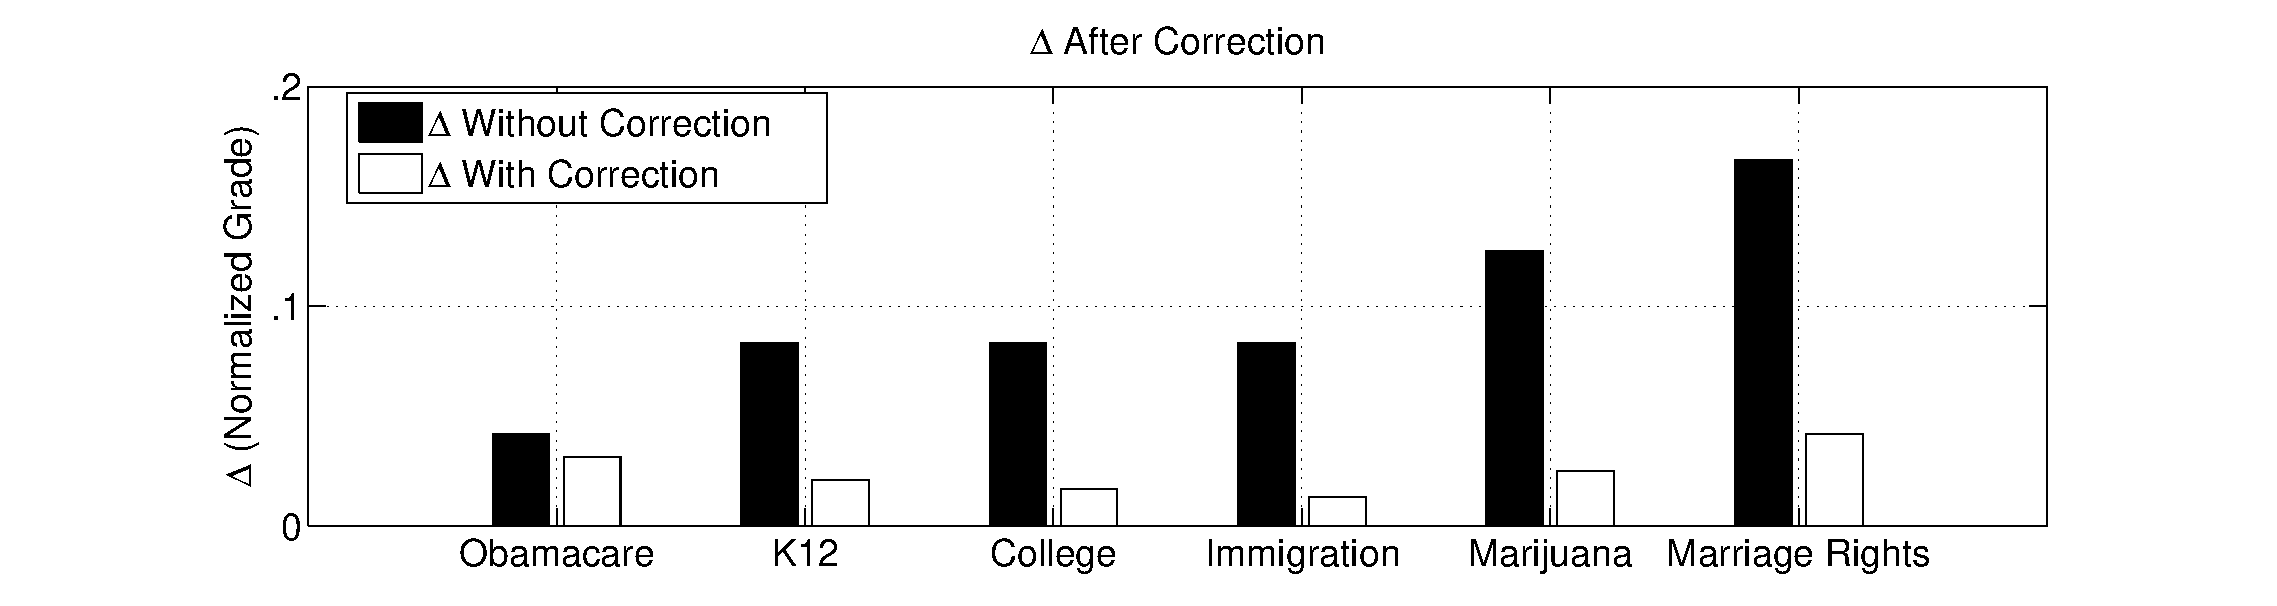
\includegraphics[scale=0.26]{../plots/shit-2.eps}
      \caption{We measured the RMSE prediction error of the polynomial model. We found that we could predict changes in all of the issues with less than 2/3 of a letter grade RMSE error. We applied this model to correct for the Social Influence bias and found that, on average, we could reduce herding effects by 46.5\%}
      \label{poly-1}
\end{figure}





\section{Future Work}
The methods we proposed have several interesting directions of future interest. 
We want to extend our work to quantify biases in textual data. 
The California Report Card collects textual suggestions from participants in addition to the quantiative assesment results. 
Participants are encouraged to read the responses of others before leaving a suggestion of their own.
We suspect that this may lead to a bias in the topics discussed by participants, and we would like to explore how similar non-parametric models can be extended to textual data.

Another compelling direction is to attempt to parameterize our model.
We will explore whether we can model the grades as a mixture of binomial distributions (a discrete analog of a mixture of gaussians), and try to derive optimal tests and models for this data.
Intuitively, parametrization should lead to increased statistical power and better fitting models; assuming that the data fits the underlying parametrization.

\section{Conclusion}
We proposed non-parametric hypothesis tests and models to evaluate the biasing tendency of visible aggregate statistics in the California Report Card.
We found that revealing the median led to a statistically significantly tighter grouping of grades around the shown median grade.

We modeled the biasing effect as a regression towards the median grade and fit polynomial to represent the functional relationship between a participant's observed difference with the median and then subsequent grade change.
We applied an information theoretic criteria to select a model of appropriate complexity.
We found that this relationship was quadratic in two out of the six issues, representing a heterogeneity in biasing for positive and negative differences with the median.
We further showed how non-parametric ideas could be extended to the problem of Wilcoxon shift parameter estimation and quantify the effects of the biasing tendency.

In principle, the methods we proposed can be applied to test and model biases in a wide variety input mechanisms.
This is a key motivation for our non-parametric approach.
Understanding these biases, can give insight into the behavior of recommender systems that train on such data.

%\end{document}  % This is where a 'short' article might terminate


%
% The following two commands are all you need in the
% initial runs of your .tex file to
% produce the bibliography for the citations in your paper.
{
\bibliographystyle{abbrv}
\fontsize{7.1pt}{7.0pt} \selectfont
\bibliography{sigproc}  % sigproc.bib is the name of the Bibliography in this case
}
% You must have a proper ".bib" file
%  and remember to run:
% latex bibtex latex latex
% to resolve all references
%
% ACM needs 'a single self-contained file'!
%
%APPENDICES are optional
%\balancecolumns

\balancecolumns
% That's all folks!
\end{document}
